\documentclass[a4paper,10pt]{article}
\usepackage[croatian]{babel}
\usepackage{hyperref}

% visual
\setlength{\parindent}{0em}
\setlength{\parskip}{.5em}

% tables
\usepackage{booktabs}
\usepackage{longtable}

% headers
\usepackage{fancyhdr}
\fancyhf{}
\usepackage[left=3cm,right=3cm,top=3cm,bottom=3cm]{geometry}

% toc font
\usepackage{tocloft}
%% naslov "sadrzaj"
\renewcommand{\cfttoctitlefont}{\Large\sc}
%% font stranica
\renewcommand{\cftsecpagefont}{\sc}
\renewcommand{\cftsubsecpagefont}{\sc}
\renewcommand{\cftsubsubsecpagefont}{\sc}
%% imena poglavlja
\renewcommand{\cftsecfont}{\sc}
\renewcommand{\cftsubsecfont}{\sc}

%index
\usepackage{makeidx}
\makeindex

\lhead{\textsc{AIRbender VR}}
\rhead{\textsc{Lekcije za stvaranje igre}}
\cfoot{\thepage}

% side notes
\usepackage{todonotes}
\usepackage{xcolor}

\pagestyle{empty}
\linespread{1.3}

\usepackage{titlesec}
\titleformat*{\section}{\Large\sc}
\titleformat*{\subsection}{\large\sc}
\titleformat*{\subsubsection}{\large\sc}

\begin{document}

\begin{center}
\textsc{Sveučilište u Zagrebu}\\
\textsc{Fakultet organizacije i informatike}\\
\textsc{Analiza i razvoj programa}
\end{center}
\vspace*{7cm}
\begin{center}
	\textsc{\huge AIRbender VR}\\
	\textsc{\large Unreal Engine}\\Naputci za izradu\\
	\vspace*{1cm}
	Dorian Čajko \quad Ivan Huzjak \quad Denis Jocković \quad  Filip
	Novački \quad Luka Štefanić
\end{center}
\hspace*{1cm}

\begin{center}\end{center}
\vspace*{7cm}

\begin{center}
VARA\v{Z}DIN
\end{center}

\pagebreak
\phantom{}
\pagebreak

\tableofcontents

\pagebreak
\phantom{}
\pagebreak

\newgeometry{top=3cm, bottom=3cm, outer=6.5cm, inner=3cm, left=3cm,
marginparwidth=4.7cm, marginparsep=0.7cm}
\pagestyle{fancy}

\section*{Uvod}

Ovaj priručnik za programiranje projekta namijenjen je prvenstveno studentima
tehničkih područja kao nit vodilja kroz stvaranje jednog projekta. Igra koja se
stvara ovim putem temelji se na popularnoj crtanoj seriji Avatar, a ime, u
originalu \textit{Avatar, the Last Airbender}, vrlo se prikladno poklopio s
imenom kolegija, \textit{Analiza i razvoj programa}, iliti skraćeno
AIR.

\index{Uvod}
Podrazumijeva se da čitatelj ovog priručnika poznaje osnovne koncepte
programiranja te se oni ovdje neće u detalje objašnjavati. Naglasak će se
staviti na koncepte koji se upotrebljavaju u izradi igre, dakle oni vezani za
Unreal Engine, razvoj igara itd.

\marginpar{\color{teal}{Dodatna objašnjenja mogu se vidjeti izdvojena sa strane
kako bi se dodatno povezalo objašnjeno s drugim konceptima.}}
Glavni tekst sadržavat će objašnjenje postupaka koji se koriste u izradi igre.
Moguće je da se koraci malo promijene u određenim verzijama softvera koji se
koriste, no pretpostavlja se da će sve ostati slično jer se ne koriste jako
opskurni koncepti.

Na kraju priručnika nalazi se kazalo pojmova kako bi se određeni pojam mogao
lakše pronaći ukoliko je samo spomenut negdje u tekstu, a nije iz naslova jasno
o kojem se pojmu točno radi.

\pagebreak

\section{Uvod u industriju, stvaranje igara te okruženje}

\begin{quote}
	\small
	Programiranje igara se po mnogočemu razlikuje od programiranja
	poslovnih aplikacija. Pristup i razmišljanje su drugačiji. Dok za
	poslovne aplikacije je važno usredotočiti se na podatke, u igrama je
	važno i misliti na tzv. \textit{delivery}, odnosno kako će korisnik
	doživjeti aplikaciju. Grafiku, fiziku, objekte i druga zajednička
	obilježja objedinjava \textit{game engine}. Unreal Engine je jedan od
	najpopularnijih rješenja za razvijanje igara te ćemo se u ovom
	priručniku koristiti njime.
	\marginpar{\small\color{teal}{
		U Unreal Engineu moguće je u potpunosti programirati u \texttt{C++}-u,
		no zbog kompleksnosti jezika i pristupačnosti
		\textit{blueprinta} uglavnom ćemo se baviti vizualnim
		skriptiranjem.
		}}

	Jedna od posebnosti Unreal Enginea je što koristi tzv.
	\textit{blueprinte}, alat kojim se odnosi između objekata programiraju
	ne kodom, nego povlaćenjem odnosa između objekata koji su
	reprezentirani vizualno što olakšava predočavanje te dodatnu razinu
	apstrakcije od programskog jezika \texttt{C++}.

	Prije nego što će biti objašnjeni detalji o Unreal Engineu objasnit će
	se i osnove dizajna video igara (en. \textit{game design}), kako teče
	proces izrade igara te na što se sve treba pripaziti kod izrade igara.
\end{quote}

Kao dodatna motivacija za stvaranje igara je činjenica da se ta industrija u
zadnjih osam godina tržišna vrijednost igara udvostručila, a predviđa se da će
se u iduće tri godine ($2020.-2023.$) vrijednost utrostručiti. Broj aktivnih
igrača u svijetu raste velikom brzinom te se u tim podatcima prepoznaje
perspektiva te industrije. Iz tog je razloga dobro poznavanje ovog sektora, ako
ne zbog želje za radom u njoj, barem zbog opće kulture.

\subsection{Dizajn video igara}

Dizajn video igara kao proces teško je definirati. Dizajn obuhvaća sve ono što
se događa za vrijeme stvaranja igre, dakle počinje idejom i temom, nastavlja
razvitkom i na kraju stvaranje verzije igre koja se izdaje i distribuira
igračima.

\paragraph{Stvaranje ideje}

Ideja se razvija na razne načine -- može doći kroz razgovor s bliskim osobama,
može se razviti kroz \textit{brainstorming}, može doći kroz bljesak
inspiracije ili na neke druge načine. Ono što je obično veći problem je doći do
jedinstvenog i kvalitetnog sadržaja jer je do dana današnjeg stvoren ogroman
broj igara.

\paragraph{Osnovne funkcionalnosti i mehanike}
\index{mehanike}

Mehanike nam govore kako će objekti međusobno
reagirati, koja je njihova interakcija, što će sve likovi raditi u igri itd.
Funkcionalnosti su alati kojim se rješavaju neki problemi, npr. kretanje
glavnog lika, obrana lika od napada, umjetna inteligencija itd.

Mehanike igre govore kako će se igra ponašati u određenim trenutcima, odnosno
na neke korisničke akcije.  Mehanike se uvelike razlikuju između različitih
žanrova i to ih često čini specifičnima. Primjeri mehanika su izazovi na
\textit{bossovima}, način na koji igrač ima interakciju s raznim objektima u
igri, kako koristi objekte, kako se objekti ponašaju prema njemu itd.
%TODO

\paragraph{Skica i razrada igre}

U ovom dijelu procesa dizajna video igre kreiraju se grube skice buduće igre i
donose se razmatranja kako će izgledati pojedini element igre. Skice nisu
detaljne, ali nam uvelike olakšavaju daljnji rad u nekom od alata. Tu se
razvijaju likovi, razine, moći itd.

\paragraph{\textit{Game Design Document}}

Nakon što je uvodni dio napravljen, vrijeme je da se pojedini elementi malo
detaljnije razrade. Taj dokument naziva se \textit{Game Design Document}, ili
kratko -- GDD. To je detaljan dokument koji, između ostalog, sadrži:

\marginpar{\color{teal}{\small U sklopu ovih lekcija neće se raditi GDD, ali za
bilo koji ozbiljan projekt dobro je imati taj dokument kao zamjenu za
dokumentaciju kako bi se olakšalo snalaženje u projektu i kodu.}}

\begin{itemize}
	\item naziv igre
	\item sažetak igre
	\item funkcionalnosti
	\item mehanike
	\item opis likova
	\item dizajn razina
\end{itemize}

Cilj dokumenta je olakšati svima razvoj igre tako da lakše zajedno surađuju. U
njemu su opisane sve glavne komponente

\subsection{VR}
\index{VR}

Igra-projekt kojeg će ovaj priručnik opisati bit će implementiran za VR.
\marginpar{\color{teal}{\small VR može vrlo lako učiniti neiskusnog igrača
omamljenog, odnosno može osjećati glavobolju, vrtoglavicu i slične simptome
ukoliko nije naviknut na virtualnu stvarnost. Postoje mnoge tehnike kako se to
može ublažiti. U ovom projektu će se pokušati voditi računa o tome koliko god
je moguće.}} VR je skraćenica na engleskom od \textit{virtual reality} što
znači da se imitira stvarnost u virtualnom okruženju. Cilj VR-a je korisniku
stvoriti osjećaj kao da je u stvarnom svijetu podražujući više osjetila.
Glavni uređaj koji je svojevrsno obilježje VR koncepta su naočale, odnosno
\textit{headset} koji prekriva cijelo vidno polje i korisniku omogućuje da vidi
sliku kao realnost tako da svako oko vidi posebnu sliku.  Ovaj projekt koristit
će i kontrolere koji omogućuju korisniku pokretanje.

Pomoću kontrolera moguće je pratiti pokrete ruku. U nekim igrama to je već
iskorišteno za precizno bacanje projektila, predmeta, uzimanje predmeta itd., a
u našem projektu to će biti glavni okidači za usmjereno bacanje moći.

\subsection{Instalacija i korištenje okruženja}

Razvojno okruženje sastoji se od Oculus softvera i Unreal engine editora.
Oculus sofrver služi kao \textit{driver} za Oculus \textit{headset}.

Postavljanje okruženja odvija se u sljedećim koracima:

\index{instalacija}
\begin{enumerate}
	\item Instalacija Oculus softvera
	\item Instalacija Unreal engine-a
	\item Pokretanje ugrađenog projekta
	\item Uklanjanje eventualnih problema
	\item Postavljanje verzionioranja na projekt
\end{enumerate}
\subsubsection{Instalacija Oculus softvera}

Za početak je potrebno  doći do Oculusove stranice
za preuzimanje softvera (\url{oculus.com/setup/}) i preuzeti
softver za uređaj na kojem razvijamo. U našem slučaju razvijamo na Oculus Rift
S i preuzimamo taj software.

\subsubsection{Instalacija Unreal Enginea}

Kako bi se instalirao Unreal Engine, potrebno je otići na mrežnu stranicu
stranicu \url{unrealengine.com}. U gornjem desnom kutu su opcije \texttt{Sign
in} te \texttt{Download}. Prijava je potrebna za pokretanje Unreal Enginea tako
da se korisnik mora registrirati prije ili kasnije.

\marginpar{\color{teal}{\small Instalacija za Linux ponešto je složenija te je potrebno kompajlirati cijeli projekt. To uzima poprilično vremena i resursa, a sadrži i
nešto više koraka koji se ovdje neće opisati jer se orijentiramo na Windows
operacijske sustave}}

Kod odabira licence potrebno je pripaziti koja se odabire. \textit{Publishing
license} ona je koja se odabire ukoliko se proizvod namjerava prodati, a
\textit{Creators license} ukoliko se namjerava raditi nemonetiziran rad.
Studenti su navedeni u obje kategorije jer se \textit{engine} ne mora plaćati
ako se koristi za projekt koji još ne stvara profit.

Dalje je potrebno registrirati se te slijediti uputstva kod instalacije. Unreal
Engine radi na operacijskim sustavima Linux te Windows.

\subsubsection{Korištenje Unreal enginea}

Dijelovi editora koji se nakon otvaranja projekta vide su:
\textit{Place Actors}, \textit{Toolbar}, \textit{Viewport},
\textit{Content Browser}, \textit{World}
\textit{Outliner} te \textit{Details panel}.

\index{place actors}
U \textit{Place Actors} dijelu se nalaze actori koji se mogu postaviti u
\textit{Viewport} jednostavnim \textit{drag'n'dropom}. Nakon kreiranja svakog
projekta u \textit{Place Actors} mogu se pronaći zadani actori koji se nalaze u
svakom projektu.

\index{viewport}
Najveći dio editora zauzima \textit{Viewport}. U \textit{Viewportu} se nalazi trenutna otvorena
razina. Svi elementi koji se u njoj nalaze mogu se označiti klikom miša. Označeni
element može se ili pomicati po sve tri osi ili se može promijeniti opcija te
se na taj način rotirati po svim trima osima.

\index{content browser}
\textit{Content browser} služi za navigaciju korisnika po raznim mapama i
dokumentima.  Iz njega se može pristupiti svim dokumentima koji se koriste u
projektu te se mogu postaviti u \textit{Viewport}.

\index{world outliner}
\textit{World Outliner} je jednostavan element editora koji se nalazi u gornjem
desnom kutu. U njemu se mogu pronaći svi \textit{actori} koji su postavljeni u
trenutno izabranom levelu. Ukoliko se odabere neki actor iz \textit{World
Outlinera}, on će automatski biti odabran i u \textit{Viewportu}.

\index{actor}
Svaki \textit{actor} koji se nalazi u \textit{Viewportu} i \textit{World
Outlineru} ima svoj \textit{Details panel. }U ovom panelu se mogu se provjeriti
i mijenjati razni podaci poput lokacije actora, rotacije, veličine. Također,
mogu se mijenjati i korištene teksture odnostno materijali, opcije kolizije
itd.

\subsection{Kreiranje projekta}

Kako bi testirali radi li cijelo okruženje ispravno učitati ćemo VR preset koji
je ugrađen u Unreal Engine. Važno je da je prije pokretanja Unreal Enginea
Oculus softver već upaljen. Pokrećemo program pritiskom na tipku "Launch" u
gornjem desnom kutu.

\marginpar{\color{teal}{\small Stvaranje prvog projekta moglo bi
potrajati znatno duže nego inače jer se mnogi resursi sad generiraju.
Dulje učitavanje može se očekivati i nakon ažuriranja na noviju verziju.}}

Za stvaranje projekta odabiremo opciju "Games" što će nas odvesti na izbornik
već izrađenih projekata koji sadrže minimalno što je potrebno kako bi se
testirale ili izrađivale dodatne mehanike.

Odabiremo "Virtual Reality" \textit{preset} u kojemu je već implementirano
kretanje, kontroleri, VR kamere, primanje objekata i kolizije. Pritiskom na
tipku "Create Project" projekt se stvara.

Kad se otvori projekt moramo odabrati kartu koja je napravljena za naš tip
uređaja za virtualnu stvarnost. Odabiremo desni preset i kartu pronalazimo u
\textit{content browseru} na dnu ekrana.

Navigiramo na lokaciju \texttt{VirtualRealityBP/Maps/MotionControllerMap} i dvostrukim klikom otvaramo tu kartu.
Po otvaranju karte u gornjoj alatnoj traci odabiremo padajući izbornik pored
tipke \textit{play}
i odabiremo \textit{VR preview}.


\begin{figure}[!h]
	\centering
	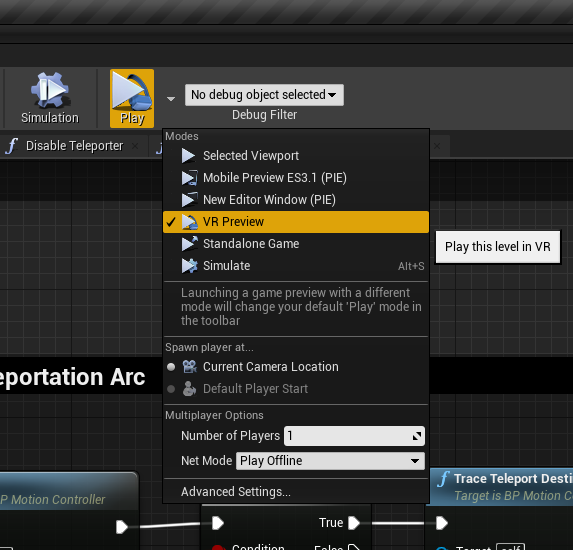
\includegraphics[width=\textwidth]{slike/R_slika7.1.png}
	\caption{Prikaz izbornika kojim se dolazi do opcije \textit{VR preview}}
\end{figure}

Ako je sve ispravno postavljeno, na uređaju bi se trebao prikazati VR pogled.



Actor je jedna od najkorištenijih klasa u Unreal Engineu. Elementi te klase su
oni koji se mogu postaviti u level. Za actore se mogu odrediti razne postavke,
primjerice kojeg će biti materijala, imaju li koliziju itd.

Klasa Pawn je podklasa Actora te ona predstavlja sve ono što korisnik može
kontrolirati. Klasa Pawn ima i svoju podklasu Character koja ima određena
svojsta koje klasa Pawn nema. Postoje još mnoge klase u UE-u međutim one nisu
toliko razvijene i korištene kao ova klasa.


U Unreal Engineu se programira prvenstveno korištenjem \textit{Blueprinta} metodom poznatom pod nazivom
\textit{Visual Scripting}. To znači da se većina koda napiše pomoću
\textit{Blueprinta} dok se
određene stvari mogu napisati i u \texttt{C++}-u. Teoretski je moguće napisati igru i u
\texttt{C++}-u, ali to se u pravilu ne radi jer je Unreal engine napravljen
tako da se dizajn igre odvaja od programiranja dijelova klasa pa se glavne
funkcionalnosti uglavnom \textit{blueprintaju}, a detalji se programiraju.

\subsection{Zaključak}

U ovom uvodu instalirali smo okruženje te se upoznali s glavnim elementima
razvijanja igara. Upoznali smo se i s pojedinostima programiranja u Unreal
Engineu te smo kontekstualizirali programiranje.

Mnogi koncepti koji vrijede u programiranju poslovnih aplikacija vrijede i u
Unrealu, kao što je verzioniranje, jedino treba posebno pripaziti na velike
datoteke i na \texttt{.gitignore}. \index{git}

Teme i koncepti kojima se može dodatno obogatiti projekt su:
\begin{itemize}
	\item verzioniranje (\texttt{git}, \texttt{LFS}...)
	\item integracija \texttt{C++} koda u \textit{blueprinte}
	\item detaljnije upoznavanje s elementima korisničkog sučelja u
		okruženju
\end{itemize}

\paragraph{Prostor za bilješke:}\phantom{}



\pagebreak
\section{Kreiranje i kretanje glavnog lika}
\index{kretanje} \index{teleportacija}

Unreal engine ima \textit{preset} za svaku popularnu vrstu video igre pa se
tako populariziranjem VR igri razvio i VR \textit{preset}. U tom
\textit{presetu} već je implementirana funkcionalnost kretanja, odnosno
teleportacije, no i dalje je važno razumjeti na koji način kretanje funkcionira
kako bi smo mogli lakše implementirati ostale funkcionalnosti u skladu s onime
što već imamo.

Kretanje je implementirano u dva odvojena objekta koji međusobno komuniciraju.
Jedan objekt je kamera kroz koji igrač prati svijet, dok je drugi objekt
kontroler, odnosno kontroleri na kojima se nalazi tipka za kretanje.

Ta su dva objekta povezana zato što se pomoću vektora kontrolera i kolizije
određuje mjesto na koje će se postaviti igrač nakon uspješne teleportacije.
Kretanje, odnosno teleportacija se izvodi kroz niz petlji.

\subsection{VR \textit{blueprint}}

Element, odnosno \texttt{actor} iz naslova je VR uređaj u virtualnom prostoru.
Taj \texttt{actor} prestavlja stvarni VR uređaj iz realnog svijeta virtualnom
svijetu. U nastavku slijedi opis svih funkcionalnosti koje su postavljene
pomoću blueprinta u navedenom actoru.

\subsubsection{Postavljanje visine igrača te postavke VR uređaja}
\index{događaj} \index{event} \index{visina} \index{postavke}

Sustav događaja je sustav koji omogućuje programerima da se neka funkcija
pokrene nakon što se nešto dogodi.

Sve što će se sada opisati okida se na događaj početka igre. Događaja  u Unreal
engineu ima mnogo. Za sada će se koristiti događaji početak igre, \textit{tick}
ili \textit{input} od strane igrača.

\begin{figure}[!h]
	\centering
	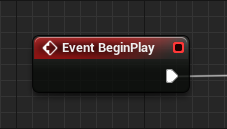
\includegraphics[]{slike/01.png}
	\caption{Događaj za početak igre}
\end{figure}

\index{PSVR}
Prvi skup čvorova koji slijedi nakon čvora početka igre služi za prilagodbu
visine igrača ukoliko se radi o PSVR \marginpar{\color{teal}{\small PSVR -- Play Station
Virtual Reality}} uređaju jer
PSVR ne zna gdje se nalazi pod te može sam odrediti visinu na kojoj se nalazi
igrač. Praćenje (eng. \textit{tracking}) \textit{headseta} i kontrolera se na
VR uređajima vrši pomoću namjanje dviju kamera koje onda mogu
uspoređivati dvije iste scene iz različitog kuta gledanja te na taj način
dobiti informacije o trodimenzionalnosti prostora kojeg pokrivaju.

Ovisno o
uređaju određuje se ime uređaja koji se kasnije koristi za indentifikaciju
scenskog elementa kojem je taj uređaj pridružen. Drugim riječima, stvarni
uređaj se veže s virtualnim te oni postaju isti element. Na taj način
pokretanjem glave koje mijenjaju lokaciju fizičkog uređaja
izazivaju i mijenjanje lokacije u virtualnom prostoru. Sljedeći čvor prikazuje
implementaciju opisanog.

\marginpar{\color{teal}{\small PSVR uređaj ima samo jednu kameru koja prati
intezivne izvore svjetlosti na PSVR uređaju te po tome može znati samo
trodimenzionanu rotaciju uređaja i nema prostornu osvještenost o poziciji samog
uređaja u odnosu na bilo koji drugi element u prostoru.}}

\begin{figure}[!h]
	\centering
	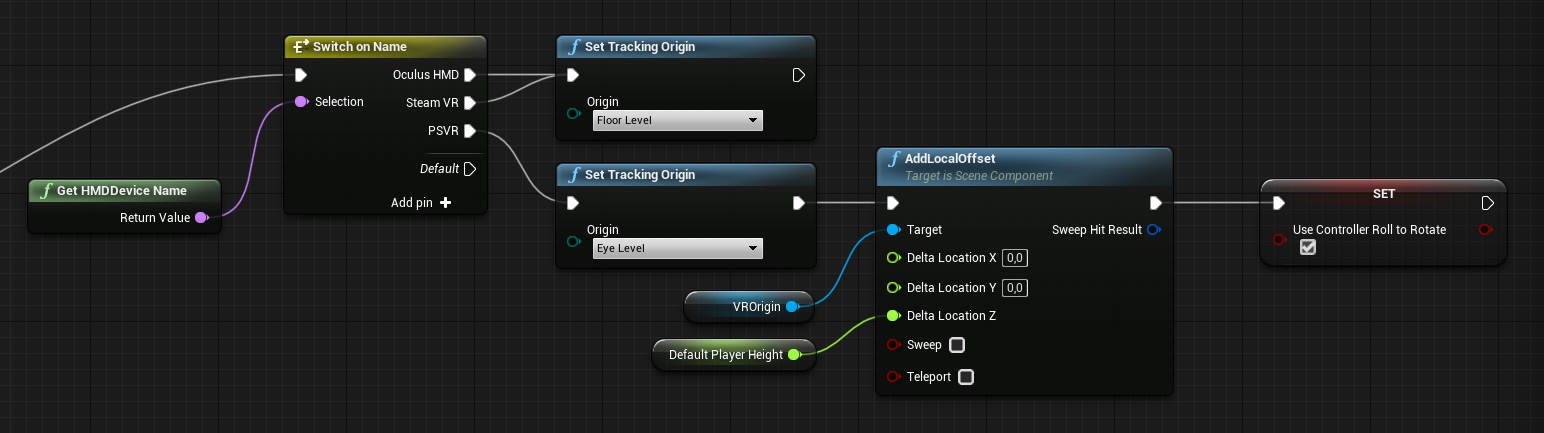
\includegraphics[width=1\textwidth]{slike/02.png}
	\caption{Čvor koji prati pokrete glave i sinkronizira pokrete s igrom}
\end{figure}

\subsubsection{Stvaranje i vezanje kontrolera za VR uređaj}

\index{PSVR}
\index{Samsung Gear VR}
\index{Google Cardboard}
\index{HTC Vive}
\index{Oculus Rift}
\index{Valve Index}
Kontroleri (ruke) nalaze se kao odvojeni \textit{actor} u Unreal Engineu kao
i u drugim \textit{game engineima} jer se kreće od pretpostavke da u projektu
može biti i samo HMD \marginpar{\color{teal}{\small HMD -- Head Mounted
Display}} \index{HMD} \index{Head Mounted Display} uređaj što obično i smatramo VR uređajem bez svojih
kontrolera. To su uređaji poput Samsung Gear VR, Google Cardboarda, spomenuti
PSVR itd. Ukoliko uređaj ima svoje kontrolere, a najpopularniji VR uređaji
poput HTC Vive, Oculus Rift S i Quest te Valve Index imaju kontrolere, onda je
te kontrolere potrebno spojiti s uređajem na način da im objekt uređaja bude
vlasnik. U nastavku se može vidjeti da se nakon početka igre stvaraju dvije
instance kontrolera koje odgovraju lijevoj i desnoj ruci.

Kod oba kontrolera
vlasnik je \texttt{Self} sto je referenca na \textit{blueprint} u kojem se trenutno izrađuju
čvorovi. Prisjetimo se da je to \textit{blueprint} od
\texttt{MotionControllerPawn}a,  odnosno
\textit{blueprint} od samog VR uređaja te ovdje sa \texttt{Self} označavamo upravo njega.
Postavljaju se vrijednosti unutar objekata \texttt{Left Controller} i \texttt{Right
Controller} te im se pridružuje roditeljska klasu koja je zapravo sam VR
uređaj. Stvaranje ruku u VR okruženju odvija se bez obzira na kolizije koje se
mogu dogoditi jer uvijek želimo da se ruke stvore iz tog razloga što su ruke na
neki način tipkovnica i miš VR uređaja uz njega samog.
\index{Controller}

\begin{figure}[!h]
	\centering
	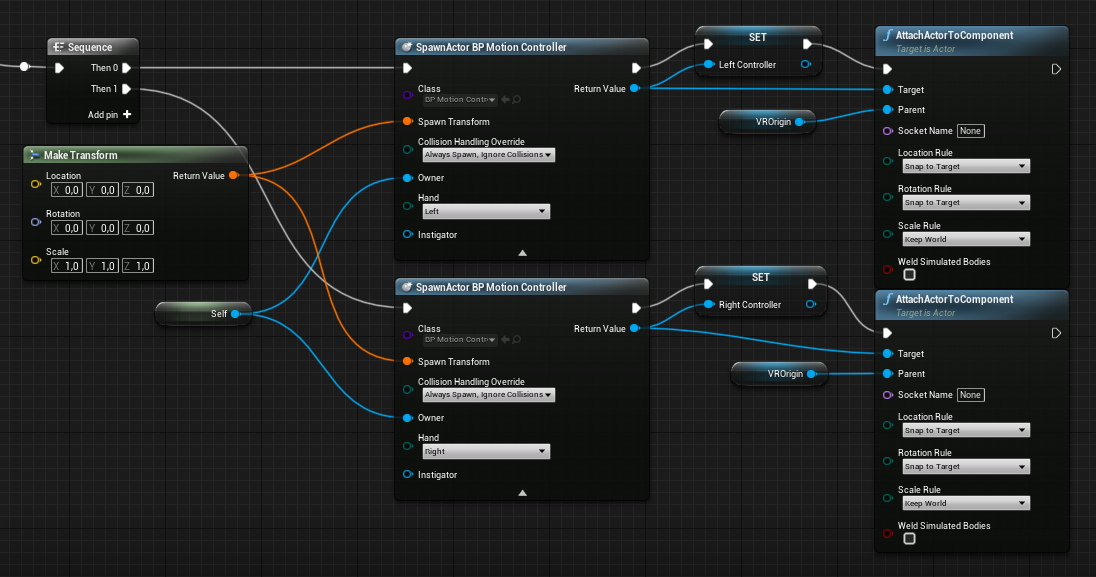
\includegraphics[width=1\textwidth]{slike/03.png}
	\caption{Pripasivanje kontrolera i HMD-a objektima}
\end{figure}

\subsubsection{Proces teleportacije}
\index{teleportacija}

Teleportacija je najkompleksniji element ove igre pa se neće moći jednostavno
prikazati i objasniti u jednom skupu čvorova. Krenut ćemo od elementa kojeg je
najjednostavnije razumjeti jer sadrži funkciju za teleportaciju. Izvršavanje
teleportacije događa se nakon provjere određenih sigurnosnih i praktičnih
uvjeta. Važno je imati u vidu
da se izvršavanje ovog dijela funkcionalnosti ne izvršava „odmah“ nakon
korisnikovog zahtjeva za teleportacijom (po pritisku tipke),
već je ovo normalan slijed operacija nakon uspješnih provjera. \textit{Odmah} je
napisano pod navodnicima jer se korisniku čini da je u tom trenutku, ali
zapravo se cijeli niz događaja odradi prije teleportacije.

U samoj funckionalnosti teleportacije postoje još dvije provjere:
\begin{itemize}
	\item nalazi li se već igrač u procesu teleportacije kada traži
		teleportaciju
	\item je li mjesto na koje se želi teleportirati valjano
\end{itemize}

Ukoliko su zadovoljena prethodna dva uvjeta zabranjuje
se prolaz novih zahtjeva za teleportaciju tako da se proces teleportacije
postavlja na vrijednost \texttt{True}. Kad je prvi uvjet zadovoljen
(\texttt{False} ovom slučaju) a drugi nije, briše se vizualna reprezentacija
teleportacije.

\index{fade out}
\index{mrak na oči}
Zadovoljavanje \marginpar{\color{teal}{fade out -- padanje mraka na oči}}oba
uvjeta pokreće funkciju koja započinje zatamnjenje (eng.  \textit{fade out})
ekrana an VR uređaju. Zatamnjenje traje isto onoliko vremena koliko traje i
funkcija odgode vremena tako da se teleportacija dogodi točno nakon potpunog
zatamnjenja ekrana.

\begin{figure}[!h]
	\centering
	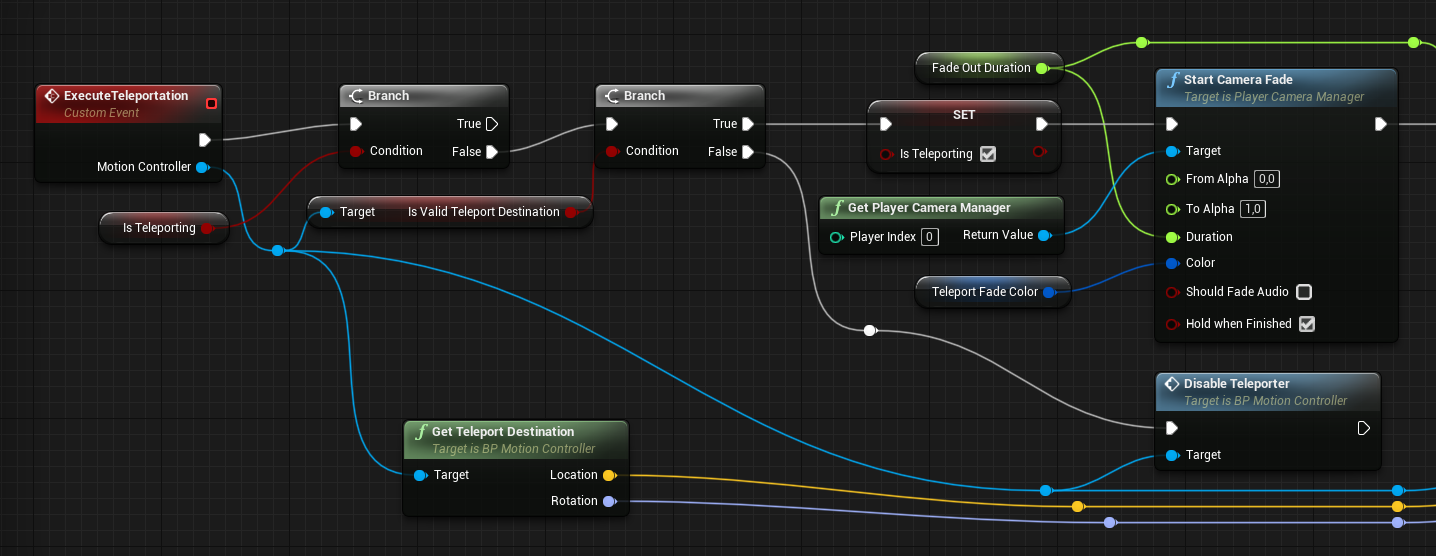
\includegraphics[width=1\textwidth]{slike/04.png}
	\caption{Prikaz procesa teleportacije}
\end{figure}


Valjano mjesto za teleportaciju ili kretanje je mjesto kojeg objekt slobodnog
\marginpar{\color{teal}{\small pawn -- realizacija igrača u virtualnom svijetu
(ne nužno u obliku čovjeka)}}
kretanja označava kao slobodnog za kretanje, a mjesto na kojeg se igrač
teleportira prikazano je indikatorom mjesta teleportacije (v. sliku
\ref{tele1}). Svaki \textit{pawn}  može imati svoj objekt slobodnog kretanja.
\index{pawn}

\begin{figure}[!h]
	\centering
	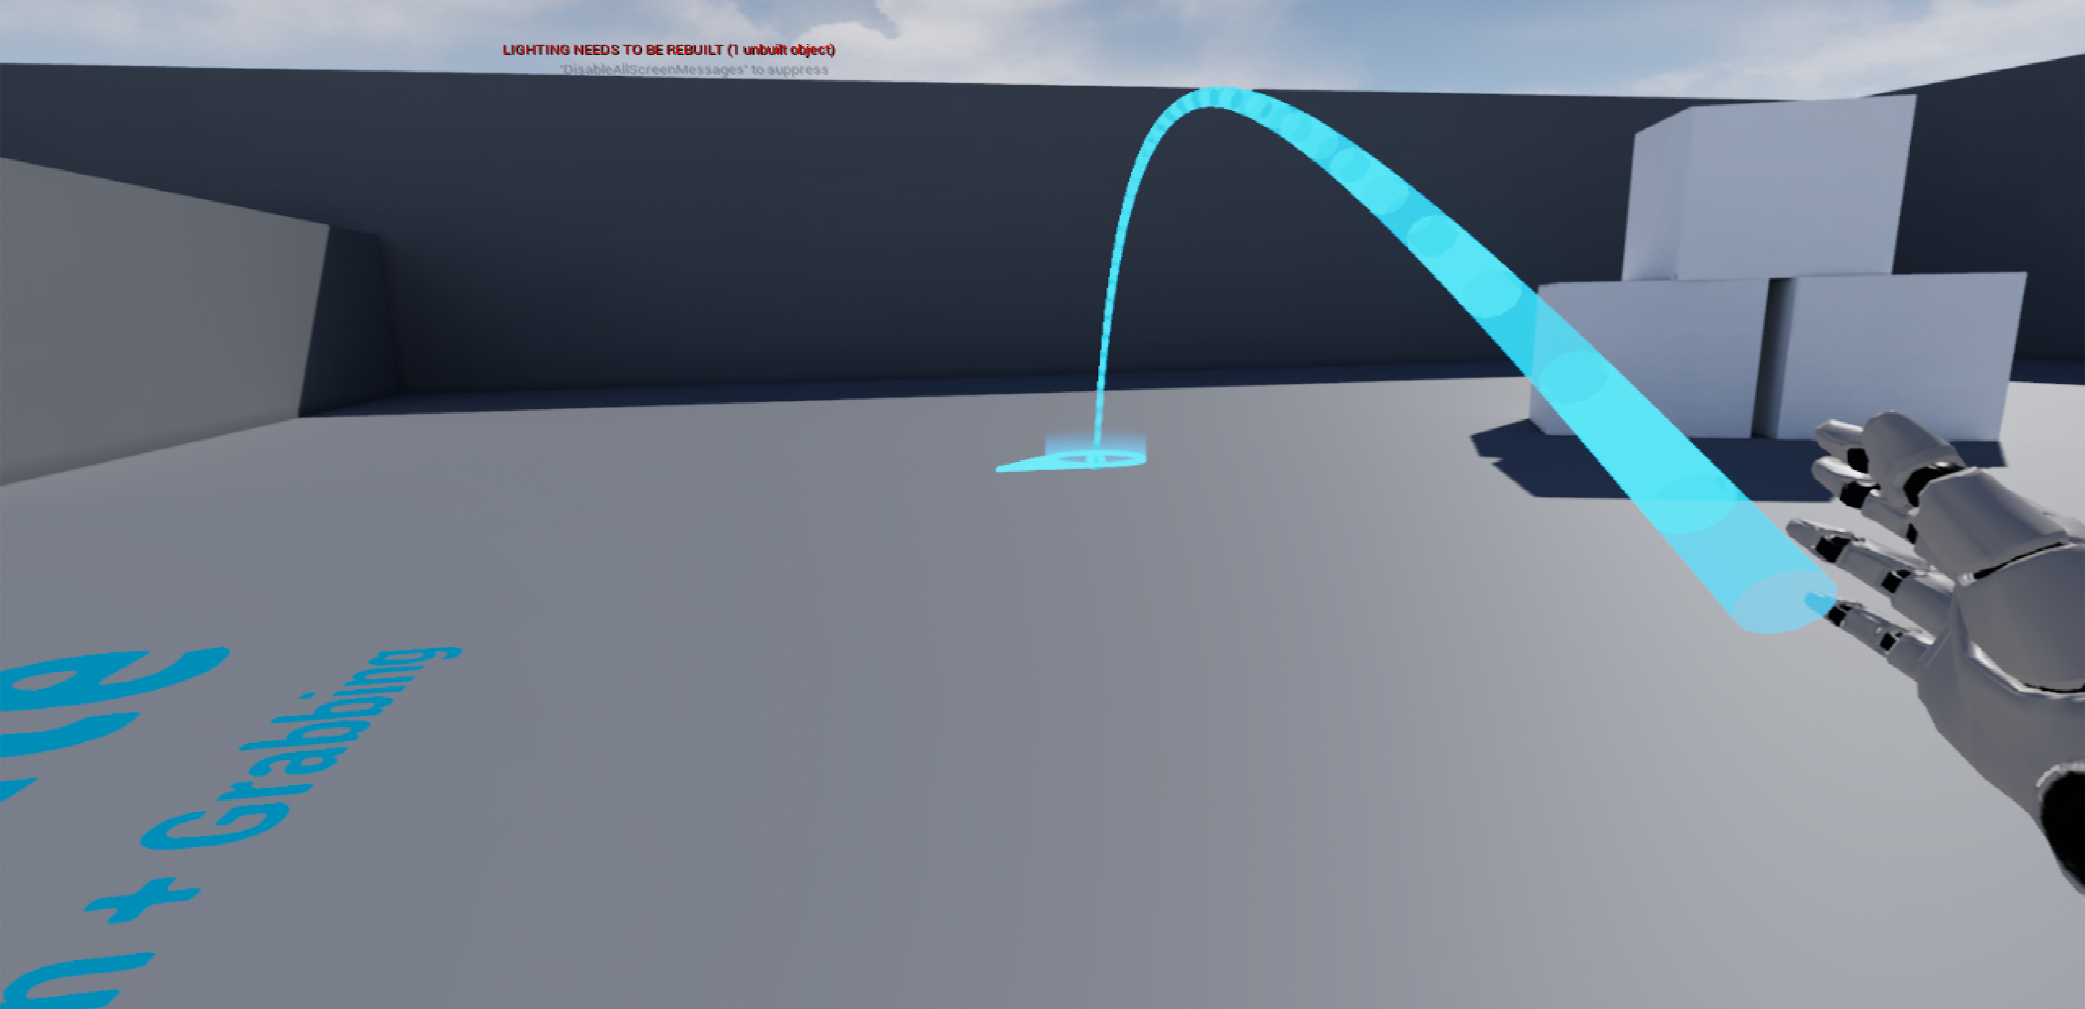
\includegraphics[width=1\textwidth]{slike/tele1.png}
	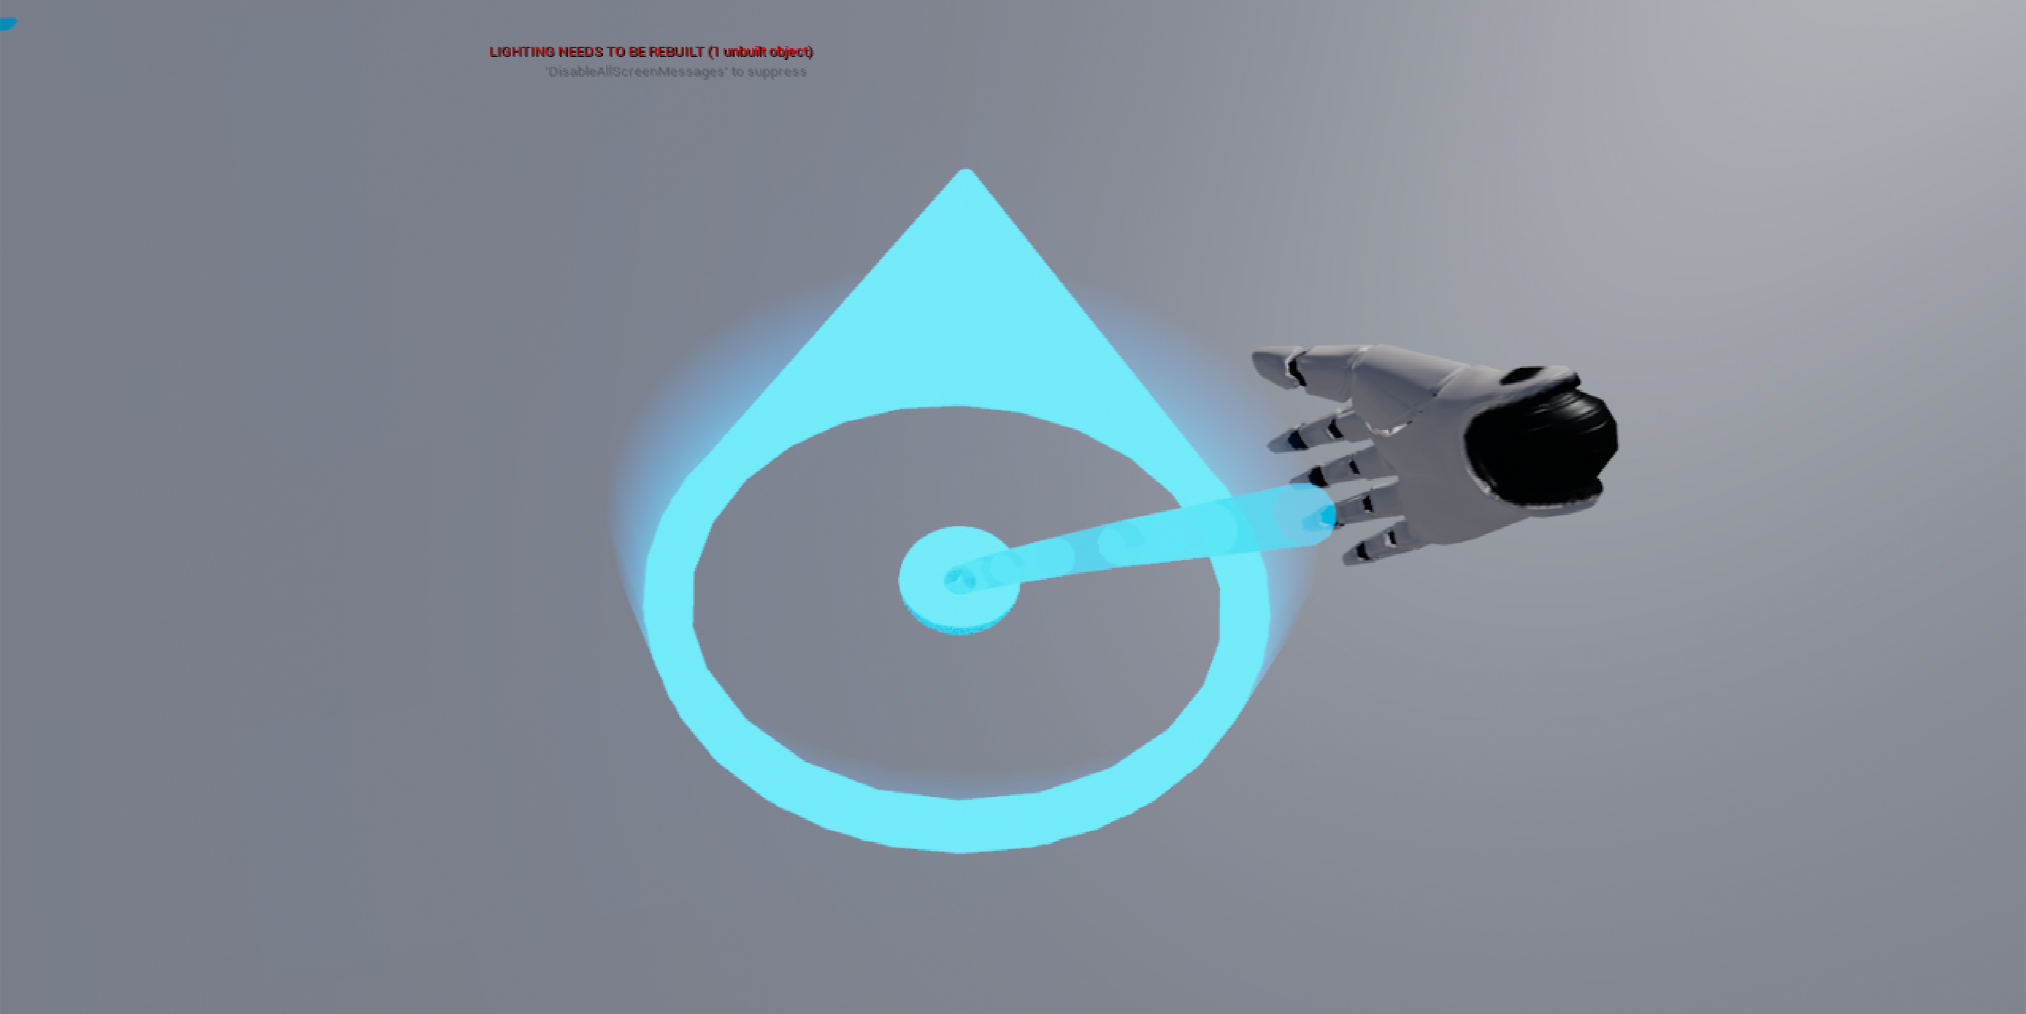
\includegraphics[width=1\textwidth]{slike/tele2.png}
	\caption{Indikator mjesta teleportacije}
	\label{tele1}
\end{figure}

Objekt zabrane kretanja su nevidljivi zidovi u videoigrama dok \textit{actor}
može biti (vidljiv) zid kroz kojeg se ne može kretati.
\index{actor}
\index{nevidljiv zid}

\index{fade in}
Nakon teleportacije započinje proces vraćanja crnog ekrana u normalan pogled
(eng. \textit{fade in}) VR uređaja. Teleportacija može bez problema raditi i bez
korištenja zatamnjenja u ove dvije spomenute funkcije i ne čini nikakvu razliku
u funkcionalnsti teleportiranja, ali poboljšava korisničko iskustvo. Obična
teleportacija bez korištenja zatamnjenja ekrana djeluje neprikladno, odnosno
igraču se može činiti kao da dolazi do grešaka. Zatamnjenje ovdje teleportaciju
čini prirodnijom koliko god se proces teleportiranja može nazvati prirodnim.

\index{indikator mjesta teleportacije}
U međuvremenu se briše vizualna reprezentacija indikatora
mjesta teleportacije i sve završava postavljanjem procesa teleportacije na
\texttt{False}. Takva zaokruženost funkcionalnosti ispitivanjem istinitosti
varijable zapravo čini jedan semafor koji ne dopušta novo izvršavanje
funkcionalnosti dok prethodno izvršavanje nije došlo do kraja. Funkcija
teleportacije lokaciju i rotaciju teleportacije dobiva od funkcije za dobivanje
željenog mjesta za teleportaciju koja se može vidjeti na prethodnoj slici.

\begin{figure}[!h]
	\centering
	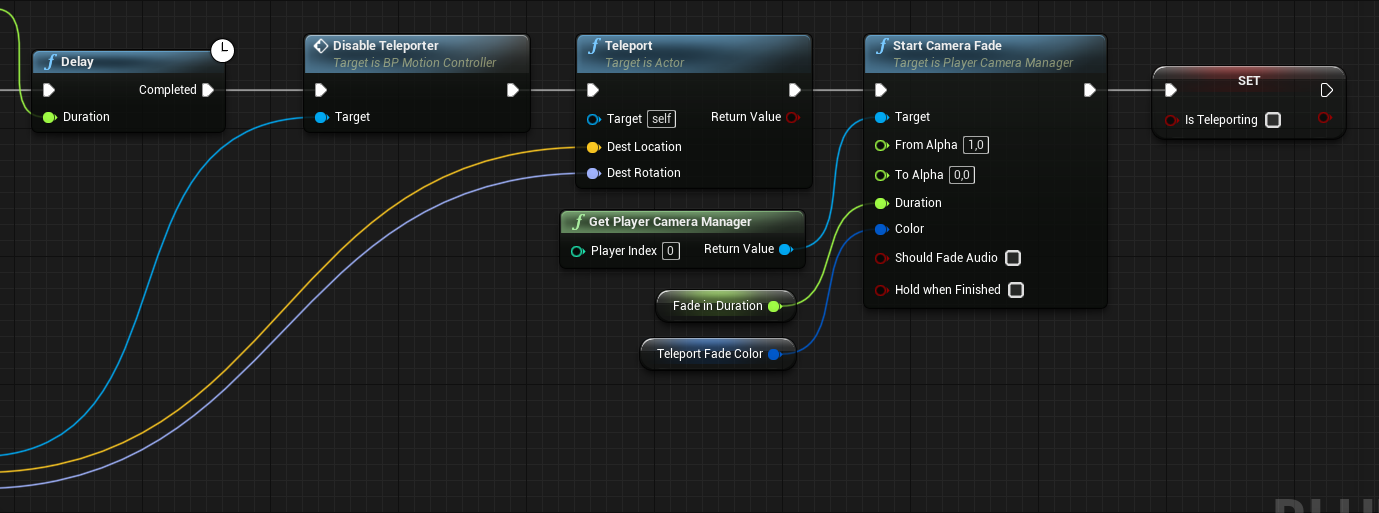
\includegraphics[width=\textwidth]{slike/05.png}
	\caption{Prikaz završetka teleportacije}
\end{figure}

\subsubsection{Rukovanje kontrolerima}

\index{kontroler}
\index{rukovanje kontrolerom}
Sljedeće funkcionalnosti okidaju se na igračev unos preko
kontrolera. Početni događaj koji to okida može se vidjeti prikazan crvenom
bojom na slici \ref{s06}. Element na kojeg utječemo je objekt kojeg smo
definirali kod spajanja kontrolera s VR uređajem. Pošto je svaki kontroler
odvojeni objekt moramo definirati što se događa i za jedan i za drugi kontroler
pritiskom na odgovarajuću tipku. Ako i na jednom i na drugom kontroleru želimo
implementirati funkcionalnost teleportacije to znači da je kod ili u ovom
slučaju skup čvorova isti osim što se referenciramo na različiti kontroler.
Zbog tog razloga će se u nastavku opisati slučaj za samo jedan kontroler jer je
implementacija za drugi kontroler manje više ista.
\index{teleportacija}

Na pritisak tipke kontrolera izvršava se
funkcija za aktivaciju teleportacije, a to je funkcija koja stvara vizualnu
reprezentaciju za mjesto teleportacije na kontroleru na kojem je pritisnuta
tipka. Nakon toga se onemogućava vizualna reprezentacija za mjesto
teleportacije na drugom kontroleru. Tako je napravljeno kako igrač ne bi mogao
izazvati grešku na način da pritisne tipku na jednom kontroleru i dok je drži
pritisnutu, pritišće tipku i na drugom kontroleru. Na ovaj način to se izbjegne
jer aktivacija na jednom kontroleru automatski znači deaktivaciju na drugom
kontroleru.

Na otpuštanje pritiska tipke provjerava se je li postavljen uvjet iz
funkcije aktivacije vizualne reprezentacije teleportacije. Ukoliko je, odlazi se
u funkciju teleportacije koju smo već opisali. Na slikama se usporedbom može
vidjeti kako se u obje slike radi o istoj funkcionalnosti te je jedina razlika
u objektu kontrolera za kojeg želimo aktivirati vizualnu reprezentaciju mjesta
teleportacije i objektu kontrolera za kojeg želimo deaktivirati vizualnu
reprezentaciju mjesta teleportacije.

\begin{figure}[!h]
	\centering
	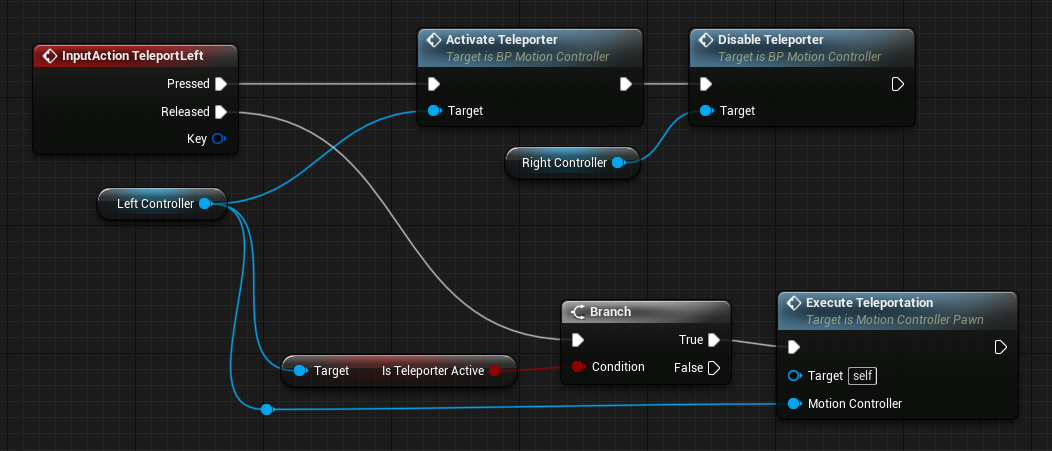
\includegraphics[width=\textwidth]{slike/06.png}
	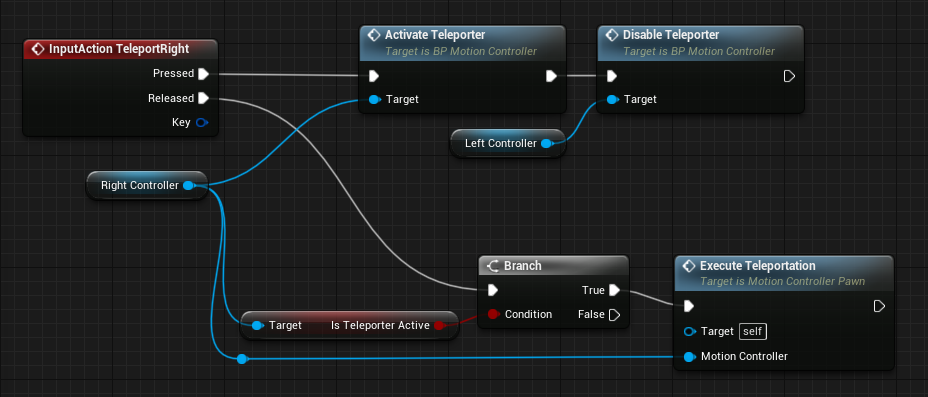
\includegraphics[width=\textwidth]{slike/07.png}
	\caption{Prikaz upravljanja kontrolerima, redom lijevi pa desni}
	\label{s06}
\end{figure}

\subsubsection{Postavljanje rotacije mjesta teleportacije}
\index{rotacija mjesta teleportacije}

Funkcionalnost koja slijedi izazvana je događajem \textit{tick} koji se konstanto
pojavljuje dok je igra pokrenuta. To je jedan od spomenutih događaja okidača
koji je također označen crvenom bojom u \textit{blueprintovima}. Iste
funkcionalnosti vrijede i za lijevi i za desni kontroler tako da se analogijom
mogu poopćiti.

\begin{figure}[!h]
	\centering
	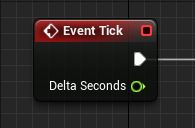
\includegraphics[]{slike/08.png}
	\caption{Slika događaja \textit{tick}}
\end{figure}

\index{gljivice}
Na objektu odabranog kontrolera ispituje se aktiviranost vizulane
reprezentacije mjesta teleportacije te ako je aktivna, postavlja se varijabla
rotacije teleportacije preko $x$ i $y$ osi na gljivici na očitanu vrijednost.
Prisjetimo se da se do ovog dijela funkcionalnosti dolazi svakim \textit{tickom} što
znači da se mogućnost promjene rotacije teleportacije događa konstantno odnosno
dokle god je valjan uvjet ulaska u petlju, a to je da je aktivirana vizualna
reprezentacija mjesta teleportacije. Isti slučaj je i kod drugog kontrolera pa
to nećemo posebno objašnjavati osim možda napomenuti očito --
razlikuje se objekt nad kojim se vrši funkcionalnost.

\begin{figure}[!h]
	\centering
	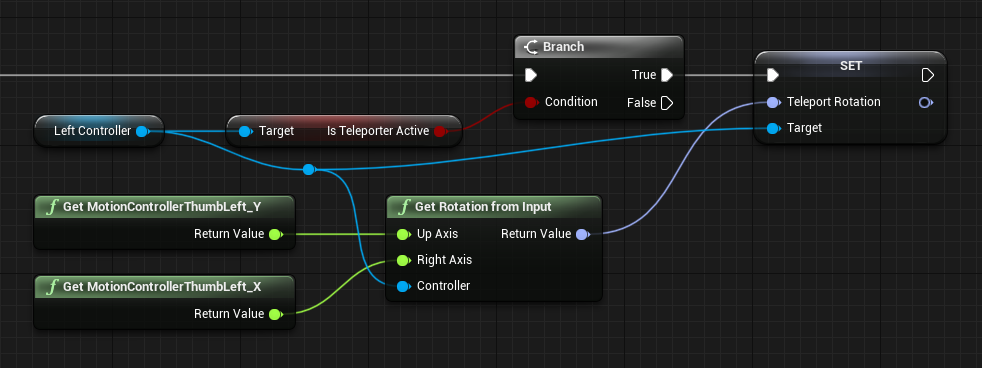
\includegraphics[width=\textwidth]{slike/09.png}
	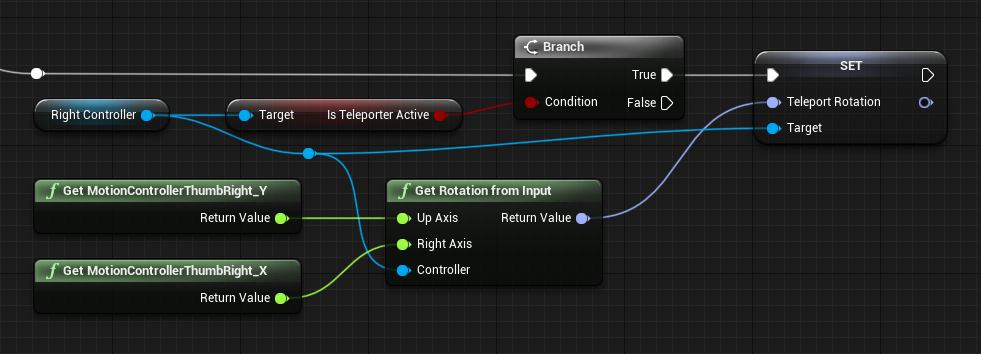
\includegraphics[width=\textwidth]{slike/10.png}
	\caption{Prikaz rotacije nakon teleportacije}
\end{figure}

\subsection{Kontroler \textit{blueprint}}

Sada prelazimo na dio koda koje se nalazi u \textit{blueprintu} od kontrolera. Prvo ćemo
krenuti od dobivanja lokacije i rotacije za mjesto teleportacije. Zbog
VR uređaja koji nemaju lokacijsku osviještenost neki su detalji malo složeniji.
\index{lokacijska osviještenost kontrolera}

\subsubsection{Dobivanje lokacije i rotacije za mjesto teleportacije}

\index{gljivice}
\index{PSVR}
Ova funkcionalnost za VR uređaje je veoma jednostavna jer se iz lokacije mjesta
teleportacije dobiva vektor lokacije te se iz postavljene rotacije preko
gljivice postavlja rotacija. Međutim, zbog kompatibilnosti sa uređajima poput
PSVR prolazi se kroz još nekoliko koraka. Uzima se trenunta pozicija VR uređaja
te se od toga uzimaju samo $x$ i $y$ vrijednosti. Zatim se taj vektor rotira prema
rotaciji gljivice te se dobiveni vektor oduzima od vektora mjesta
teleportacije. Ovo se ponovo izvršava u svrhu prilagođavanja VR uređaju koji ne
poznaje visinu jer je na ovakav način visina nebitna te će se postaviti na onu
prijašnje utvrđenu udaljenost od poda kao novu visinu.

\begin{figure}[!h]
	\centering
	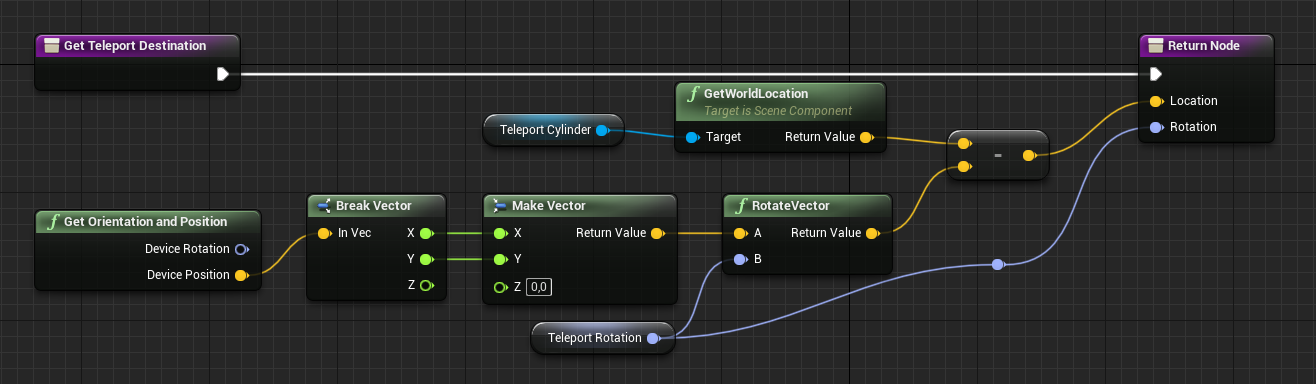
\includegraphics[width=\textwidth]{slike/11.png}
	\caption{Prikaz rotacije nakon teleportacije}
\end{figure}


\subsubsection{Aktiviranje vizualizacije mjesta teleportacije}

Poziv ove funkcije već smo koristili kod pritiska tipke kontrolera na
\textit{blueprintu} VR uređaja. Ova funkcija postavlja istinitost varijable
aktivacije
vizualizacije mjesta teleportacije na \texttt{True} te postalja vidljivost strelice
koja vizualizira lokaciju i rotaciju na vidljivo. Jednostavnost i briljantnost
ovog skupa čvorova može se vidjeti na slici \ref{s12}.

\begin{figure}[!h]
	\centering
	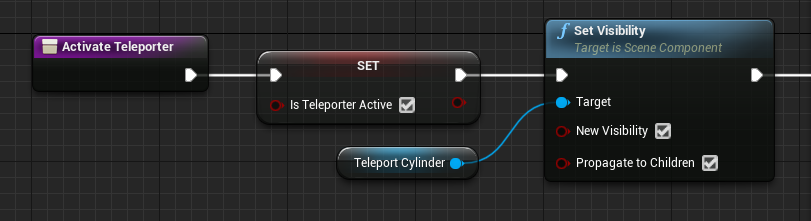
\includegraphics[width=\textwidth]{slike/12.png}
	\caption{Prikaz prikaza vizualizacije mjesta teleportacije}
	\label{s12}
\end{figure}

\index{light-house praćenje}
Postoje i dodatne funkcionalnosti koje nisu potrebne za normalno funkcioniranje
teleportacije na Oculus Rift S uređaju, no za neke druge uređaje je korisno. Svi
VR uređaji koji koriste \textit{light-house} praćenje mogu se poslužiti i vidljivosti
scenske komponente koja je prostor u kojem se igra. Ovdje to ne možemo ispitati
pa nećemo detaljnije ni obrađivati. Još jedna dodatna funkcionalnost koja je
pračenje rotacije kontrolera odnosno zapešća. Ova rotacija se može korisititi u
igrama, ako želimo da igrač određuje rotaciju teleportacije preko rotacije
kontrolera odnosno svojeg zapešća. Nekada može biti zanimljivo no više je
umrajaće od rotacije preko gljivice zato što je neprirodno te ga mi nećemo
koristiti. Ovdje se može vidjeti opisani dio.

\begin{figure}[!h]
	\centering
	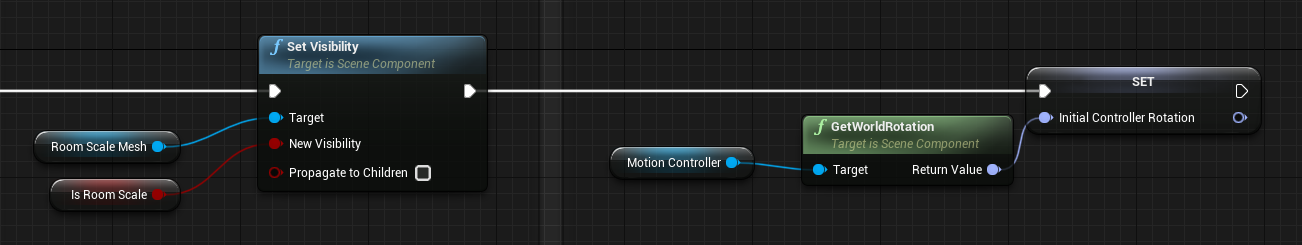
\includegraphics[width=\textwidth]{slike/13.png}
	\caption{Aktivacija indikatora mjesta teleportacije}
\end{figure}


\subsubsection{Dektiviranje vizualizacije mjesta teleportacije}

\index{indikator mjesta teleportacije}
\index{inside-out praćenje}
\marginpar{\color{teal}{ \small Oculus Riftovi imaju tzv. \textit{inside-out}
praćenje što znači da za praćenje fizičke pozicije kontrolera i samog VR
uređaja nisu potrebni vanjski elementi tj.  \textit{light-house} na dva
suprotna kraja prostora za igru. VR uređaji koji koriste \textit{inside-out}
praćenje imaju kamere na samom VR uređaju koje preko izraženih točaka u
stvarnom prostoru poput ruba stola, točke nagle promjene u boji tepiha i sl.
određuju vlastite točke praćenja u stvarnom svijetu te na taj način određuju
fizičku poziciju VR uređaja i kontrolera što se na kraju preslikava i u
virtualno okruženje.}}

\index{room-scale}
Funcionalnosti koja uklanja vizualizaciju mjesta teleportacije je ona koja je
također potrebna kako se vizualizacija ne bi stalno vidjela. Kako smo
vrijednost varijable aktiviranosti vizualizacije teleportacije postavili na
\texttt{True}, ovdje provjeravamo tu varijablu te ju postavljamo na
\texttt{False}.  Na taj način provjeravamo je li igrač ušao u proces aktivacije
jer se ne bi smjelo ništa isključiti ako nije uključeno.  Postavlja se
vidljivost indikatora lokacije i rotacije na nevidljivo isto kao i vidljivost
kraja luka za teleportaciju. Na kraju se postavlja vidljivost za \textit{room
scale} element koji ponovo nemamo kod našeg VR uređaja, no zbog kompatibilnosti
ćemo ga samo spomenuti.

\begin{figure}[!h]
	\centering
	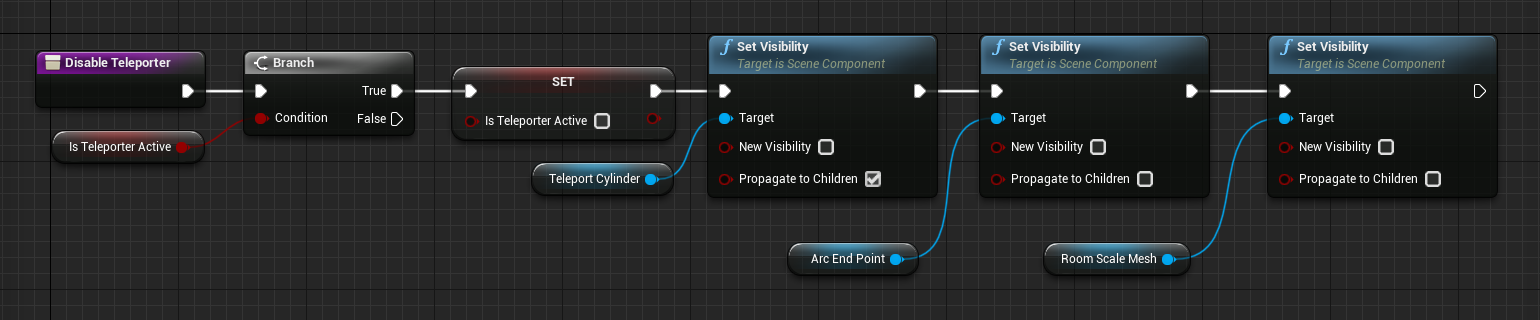
\includegraphics[width=\textwidth]{slike/14.png}
	\caption{Deaktivacija vizualnog indikatora mjesta teleportacije}
\end{figure}


\subsection{Zaključak}

Kroz ovu lekciju pokazali smo kako funkcioniraju osnovne funkcionalnosti
kretanja u prostoru pomoću VR uređaja te kontrolera. Ove pretpostavljene
funkcionalnosti napravljene su tako da većina VR uređaja radi na
\textit{plug'n'play} način te tako da se ne moraju stalno iznova programirati
osnovne stvari.

Kao dopunu ove lekcije korisno bi bilo i istražiti koncepte:
\index{light-house praćenje}
\index{rotacija zapešća}
\begin{itemize}
	\item \textit{light-house} praćenje i \textit{inside-out} praćenje
	\item \textit{room-scale}
	\item praćenje rotacije zapešća za smjer teleportacije umjesto gljivice
		-- ponekad neprirodno, ali korisno za istražiti
\end{itemize}
\paragraph{Prostor za bilješke:}\phantom{}


\pagebreak
\section{Detekcija pokreta kontrolera}

\pagebreak
\section{Stvaranje meta}

\pagebreak
\section{Napadačke moći}

\pagebreak
\section{Stvaranje prijetnji za igrača i prikaz zdravlja (HP)}

\pagebreak
\section{Obrambeni mehanizmi za igrača}

\pagebreak
\section{Bodovanje i prikaz bodova}

\pagebreak
\section{Izrada krajolika nivoa}

\pagebreak
\section{Izbornici}

\pagebreak
\section{"Umjetna inteligencija" -- protivnik se kreće}

\pagebreak
\section{Vizualni efekti}

\pagebreak
\section{Zvuk}

\printindex
\end{document}
